\chapter{Rationale Agenten}
\section{Eigenschaften Rationale Agenten}
Ein rationaler Agent ist ein System mit folgenden 4 Eigenschaften, resp. Fähigkeiten:
\begin{enumerate}
	\item Es kann die Umwelt wahrnehmen
	\item Observationen werden eingesetzt um Entscheidungen zu fällen
	\item Entscheidungen resultieren in einer Aktion
	\item Alle Entscheidungen sind rational
\end{enumerate}

Der letzte Punkt bedeutet, dass immer die Option gewählt wird, bei dem das System den meisten Nutzen hat. Das heisst also, dass ein rationaler Agent ein Belohnungssystem haben muss. Rationales Verhalten kann somit durch rationales Denken erreicht werden.

Wenn die Umwelt aber komplex ist, wird es schwierig, alle nötigen Informationen zu verarbeiten, weswegen man in diesen Situationen auch von 'eingeschränkter Rationalität' spricht.

\begin{figure}[h!]
\centering
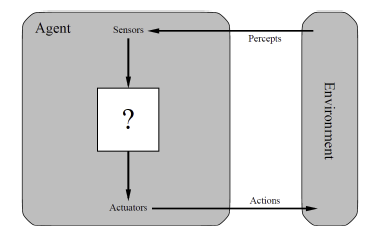
\includegraphics[width=0.4\linewidth]{fig/rationaler_agent}
\caption{Übersicht Aufbau rationaler Agent}
\label{fig:rationaler_agent}
\end{figure}

Wie in Abbildung \ref{fig:rationaler_agent} gezeigt, nimmt ein Agent Informationen über seine Umgebung mit Sensoren auf, verarbeitet diese irgendwie (dargestellt  durch das Fragezeichen) und reagiert darauf über seine Aktoren.

\section{Beispiele für rationale Agenten}
Ein Mensch hätte also z.B. Augen, Tastsinn \& Geruchssinn als Sensoren, und Arme / Beine oder Sprache als Aktoren. Das Gehirn wäre seine Kognition.

Ein Saugroboter wie in Bild \ref{fig:saugroboter} könnte z.B. wahrnehmen, ob er in Feld \textit{A} oder \textit{B} ist und könnte feststellen, ob das aktuelle Feld dreckig ist oder nicht. Er könnte dann als Aktionen entweder Saugen, das Feld wechseln oder auch nichts tun.

\begin{figure}[h!]
	\centering
	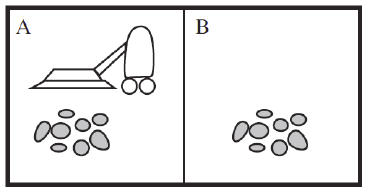
\includegraphics[width=0.4\linewidth]{fig/saugroboter}
	\caption{Rationaler Agent Saugroboter}
	\label{fig:saugroboter}
\end{figure}

\section{Modellierung / Struktur}
Alle Agenten, die man modelliert, haben folgende Eigenschaften: Sie haben eine \textbf{Sequenz von Informationen} über ihre Umgebung. Dabei muss man sich entscheiden, ob er auch irgendwann etwas vergisst. Das zweite ist die \textbf{Agenten Funktion}. Sie beschreibt das Mapping von einer Sequenz von Informationen über die Umgebung zu einer Aktion. Das \textbf{Agenten Programm} ist dann die Implementation von der Agenten Funktion und für jeden Agenten natürlich spezifisch. Die \textbf{Architektur} eines Agenten bietet Schnittstelen zur Umgebung (Aktionen / Sensoren).

Agenten haben zudem folgende Teilprogramme:
\begin{itemize}
	\item \textbf{Erkundung} Der Agent nimmt Informationen über die Umgebung auf durch Erkundungs-Aktionen.
	\item \textbf{Lernen} Der Agent lernt über Beobachtungen dazu.
	\item \textbf{Autonomie} Der Agent kann mit falschen oder unvollständigen Informationen umgehen.
\end{itemize}

\section{Performance}
Die Leistung (Performance) eines rationalen Agenten misst man \textit{von aussen} mittels Bewertungskriterien. Beispielsweise für den Staubsauger-Agenten - Quadratmeter pro Stunde, Energieverbrauch, ...  Man misst sie von aussen, weil die gewählten Aktionen eines Agenten Einfluss auf die Umgebung haben kann, oder eben auch nicht. Das kann der rationale Agent ja auch gar nicht wissen.

Eine optimale Leistung ist oft unerreichbar - zu komplexes Problem oder alle benötigten Informationen sind nicht verfügbar. Daher kann ein rationaler Agent mittels seines Wissens und seiner Beobachtungen nur die \textit{erwartete} Performance maximieren. Ein \textbf{allwissender Agent} hingegen kann auch die \textit{reale} Performance verbessern - weil er ja genau weiss, was passieren wird wenn er Aktion X ausführt.

\subsection{Definition}
Für jede mögliche Sequenz von Beobachtungen soll ein rationaler Agent eine Aktion auswählen, welche basierend auf seinen Beobachtungen und Wissens die erwartete Performance maximiert.

\section{Umgebungen}
Für jeden Agenten sind natürlich folgende Eigenschaften definiert;
\begin{enumerate}
	\item Sensoren
	\item Aktoren
	\item Umgebung
	\item Bewertungskriterium
\end{enumerate}

Die Umgebung kann nach folgenden Eigenschaften charakterisiert werden;

\begin{description}
	\item[Zugänglich vs. Unzugänglich] Ist die Umgebung für die Sensoren zugänglich? d.h. können alle relevanten Aspekte der Umgebung von Sensoren erfasst werden?
	\item[Deterministisch vs. Stochastisch] Deterministisch meint, dass der nächste Zustand der Umgebung komplett von der Aktion des Agenten abhängig ist. Stochastisch bedeutet, dass sie der Realität entspricht.
	\item[Episodisch vs Sequentiell] Episodisch bedeutet, dass die Qualität einer Aktion nur anhand der aktuellen Perzeption der Umgebung bestimmt ist - d.h. z.B. das Sortieren von Objekten. Sequentiell wäre das Spielen von Schach - dort ist die aktuelle Aktion abhängig von der vorherig gewählten.
	\item[Statisch vs. Dynamisch] Verändert sich die Umgebung während der Agent überlegt?
	\item[Diskret vs. Kontinuierlich] Ist die Umgebung diskret (Schachspiel) oder kontinuierlich (Roboter bewegt sich im Raum)?
	\item[Einzel-Agent vs. Multi-Agent] Gibt es mehrere Agenten? Sind sie konkurrierend / kooperierend?
	\item[Wissend vs. Unwissend] Wie viel weiss der Roboter zu Beginn?
\end{description}

\section{Typen von Agenten}
\subsection{Simple Reflex}
\begin{figure}[h!]
\centering
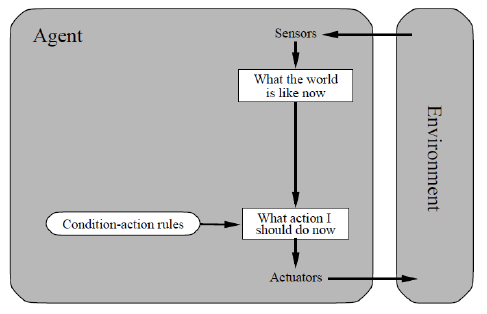
\includegraphics[width=0.5\linewidth]{fig/reflex_agent}
\caption{Reflex Agent}
\label{fig:reflex_agent}
\end{figure}
Reflex Agenten nehmen den Input aus der Welt, interpretieren ihn (z.B. bei Video-Bildern) und leiten daraus ihre nächste Aktion ab. z.B. Auto bremst - ich bremse. Heisse Herdplatte - Hand weg.

Es können so auch unendliche Wiederholungen entstehen, wenn die Umgebung nicht ganz-erfassbar ist. Das ist lösbar mittels Zufallsgeneratoren. So kann ein Staubsauger, der einfach immer nach links gehen würde, auch einmal nach rechts gehen. Siehe als Übersicht auch Abbildung \ref{fig:reflex_agent};
\subsection{Model-based Reflex Agent}
\begin{figure}[h!]
\centering
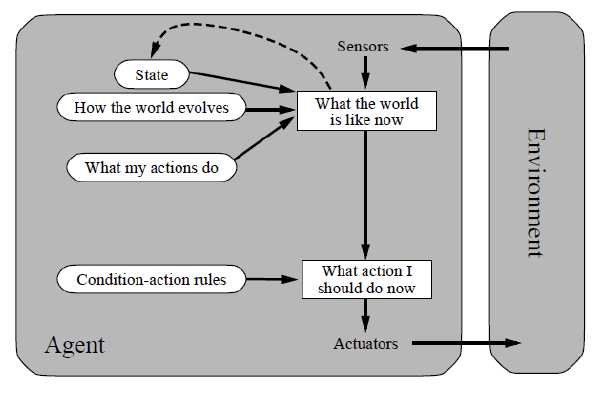
\includegraphics[width=0.5\linewidth]{fig/model_agent}
\caption{Model Agent}
\label{fig:model_agent}
\end{figure}
Der Model-based Reflex Agent speichert zusätzlich noch sein \textbf{internes Welt-Modell} ab (das ist natürlich abhängig von dem, was er bereits 'gesehen' hat), weiss in etwa, was der\textbf{ Effekt seiner Aktionen }sind und wie sich die \textbf{Welt zirka verändern wird}. 

\subsection{Goal-Based}
Wahnsinn, jetzt weiss ich, wie sich die Welt verändert. Was will ich aber genau? Was ist der Sinn des Lebens? Was sind meine Ziele? 

Das hat der \textit{Goal-based Agent} nämlich - Ziele. Es evaluiert jetzt einfach zusätzlich noch, wie sich seine Aktionen auf das Erreichen seines gewünschten Ziels auswirken wird.
\begin{figure}[h!]
\centering
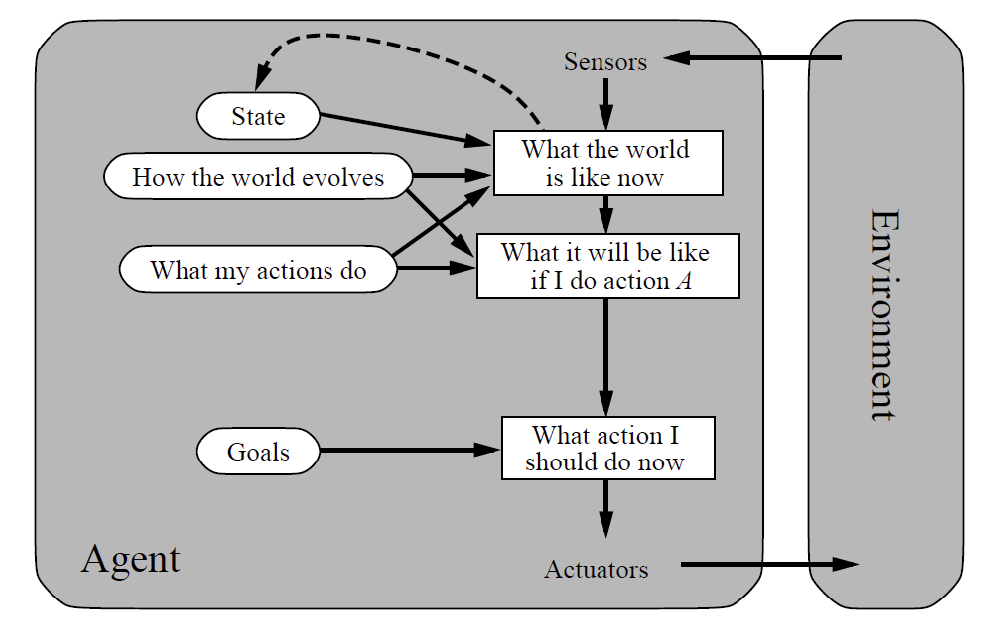
\includegraphics[width=0.5\linewidth]{fig/goal_agent}
\caption{Goal Based}
\label{fig:goal_agent}
\end{figure}

\subsection{Utility-Based}
Wenn jetzt mehrere Varianten zur Verfügung stehen, kann der Agent mit seiner \textit{utility-Funktion} entscheiden, welche dieser Aktionen ihm am meisten nützt.
\begin{figure}[h!]
\centering
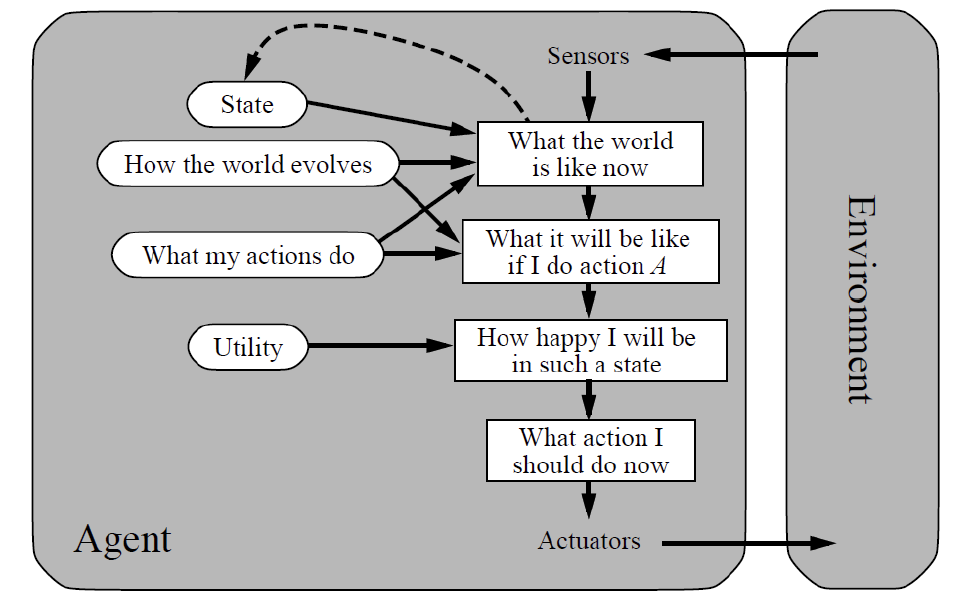
\includegraphics[width=0.5\linewidth]{fig/utility_agent}
\caption{Utility Agent}
\label{fig:utility_agent}
\end{figure}

\subsection{Learning}
Lernende Agenten starten mit einer unbekannten Umgebung und ohne Wissen. Sie haben ein \textbf{learning element}, mit dem sie Verbesserungen am \textbf{performance element} ausführen, welches zuständig ist für die Auswahl von Aktionen. Der \textbf{critic} ist etwas externes, dass die Performance des Agenten bestimmt. Der \textbf{problem generator} bestimmt auch Aktionen, mit denen der Agent etwas dazulernen kann, er stellt sich also selbst Aufgaben, damit er testen kann ob das gut war oder nicht.
\begin{figure}[h!]
\centering
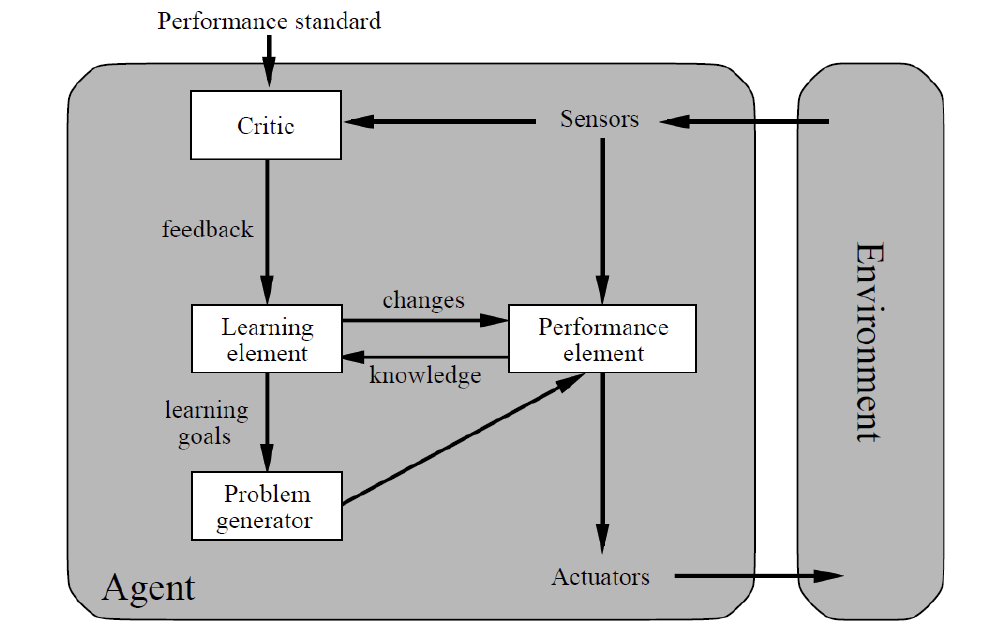
\includegraphics[width=0.5\linewidth]{fig/learning_agent}
\caption{Learning Agent}
\label{fig:learning_agent}
\end{figure}

\subsection{Lernfragen}
\begin{enumerate}
	\item Was ist ein rationaler Agent?
	\item Wie können wir Umgebungen charakterisieren?
	\item Welche Typen von rationalen Agenten unterscheiden wir? Was können Sie?
\end{enumerate}